% ============================================================================
% MAINTIDOC --- PROJECT PRESENTATION
% ============================================================================

\documentclass[aspectratio=169]{beamer}

% ----------------------------------------------------------------------------
% 1. COMPATIBLE ENGINE AND PACKAGES
% ----------------------------------------------------------------------------
\usepackage{iftex}
\ifPDFTeX
  \usepackage[utf8]{inputenc}
  \usepackage[T1]{fontenc}
  \usepackage{lmodern}
\else
  \usepackage{fontspec}
  \defaultfontfeatures{Ligatures=TeX}
  \setsansfont{Latin Modern Sans}
\fi

\usepackage{textpos}
\usepackage{graphicx}
\graphicspath{{./}{assets/}{assets/logos/}{assets/images/}{assets/user/}}
\usepackage{wrapfig}
\usepackage{tikz}
\usetikzlibrary{arrows.meta,backgrounds,calc,fit,matrix,positioning,shapes.geometric,shapes.symbols}
\usepackage{amsmath,amssymb}
\usepackage[framemethod=TikZ]{mdframed}
\usepackage{caption}
\usepackage{array}
\usepackage{colortbl}
\usepackage{pgfgantt}
\usepackage{pgf-umlsd}
\usepackage{listings}
\usepackage{adjustbox}
\usepackage{xparse}
\hfuzz=3pt

\usetheme{Boadilla}
\usecolortheme{default}
\setbeamercolor{structure}{fg=blue!65!black}
\setbeamercolor{alerted text}{fg=red!75!black}
\setbeamercolor{block title}{bg=blue!12,fg=black}
\setbeamercolor{block body}{bg=blue!3,fg=black}
\setbeamertemplate{caption}[numbered]
\setbeamertemplate{navigation symbols}{}

% ----------------------------------------------------------------------------
% 2. PERMANENT VISUAL SYSTEM
% ----------------------------------------------------------------------------
\tikzset{
  actor/.style={draw, ellipse, minimum height=1.5em, minimum width=3em, align=center},
  usecase/.style={draw, ellipse, minimum height=2.5em, minimum width=3.2cm, align=center},
  stage/.style={draw, thick, rounded corners=4pt, minimum width=2.5cm,
                minimum height=1.25cm, inner sep=5pt, align=center, font=\small\bfseries},
  component/.style={draw, rounded corners=3pt, minimum width=2.15cm,
                    minimum height=0.9cm, align=center, font=\scriptsize},
  datastore/.style={draw, cylinder, shape border rotate=90, aspect=0.28,
                    minimum width=1.9cm, minimum height=1.05cm, align=center, font=\scriptsize},
  boundary/.style={draw, dashed, rounded corners=5pt, inner sep=9pt},
  flow/.style={-{Latex[length=2.5mm]}, thick, draw=gray!75!black},
  criticalflow/.style={-{Latex[length=2.8mm]}, very thick, draw=red!75!black},
  note/.style={font=\tiny, text=gray!80!black, align=center},
  decision/.style={draw, diamond, aspect=2.2, align=center, font=\scriptsize},
  result/.style={draw, rounded corners=5pt, fill=green!12, minimum width=2.3cm,
                 minimum height=1cm, align=center, font=\scriptsize\bfseries}
}

\newcommand{\pertnode}[6]{%
  \node[draw, thick, minimum width=2cm, minimum height=1.15cm,
        fill=white, inner sep=0pt, outer sep=2pt, #2] (#1) at #3 {};%
  \node[font=\scriptsize\bfseries, anchor=center]
        at ([yshift=0.18cm]#1.center) {#4};%
  \draw[thick] ([yshift=-0.08cm]#1.west) -- ([yshift=-0.08cm]#1.east);%
  \draw[thick] ([yshift=-0.08cm]#1.center) -- (#1.south);%
  \node[font=\tiny, anchor=center]
        at ([xshift=-0.5cm, yshift=-0.36cm]#1.center) {#5};%
  \node[font=\tiny, anchor=center]
        at ([xshift=0.5cm, yshift=-0.36cm]#1.center) {#6};%
}

\newcommand{\slidepurpose}[2]{%
  \vspace*{-0.23cm}
  \begin{center}
  {\tiny
  \setlength{\fboxsep}{3pt}%
  \setlength{\fboxrule}{0.6pt}%
  \fcolorbox{black!55}{gray!10}{%
  \parbox{\dimexpr0.97\linewidth-2\fboxsep-2\fboxrule\relax}{\raggedright
  \textbf{Role:} #1 \hfill \textbf{Project Stage:} #2}}}
  \end{center}
  \vspace{0.03cm}
}

\newcommand{\defitem}[2]{\textbf{#1}: #2\par\vspace{0.32em}}

\newcommand{\placeholdergraphic}[2][0.62\textheight]{%
  \fbox{\begin{minipage}[c][#1][c]{0.88\linewidth}
  \centering\small\textbf{Asset placeholder}\\[0.25cm]
  \texttt{#2}
  \end{minipage}}
}

\newcommand{\solutionfigure}[2]{%
  \begin{center}
  \begin{minipage}[c][0.67\textheight][c]{\linewidth}
  \centering
  \IfFileExists{#1}{%
    \includegraphics[width=0.98\linewidth,height=0.61\textheight,keepaspectratio]{#1}%
  }{\placeholdergraphic[0.51\textheight]{#1}}
  \end{minipage}
  \vspace{0.06cm}
  {\captionsetup{type=figure,font=tiny,justification=centering}
  \captionof{figure}{#2}%
  \addcontentsline{lof}{figure}{\protect\numberline{\thefigure}{#2}}%
  \recordfigureentry{#2}}
  \end{center}
}

\newcommand{\tikzsolutionfigure}[2]{%
  \begin{center}
  \begin{minipage}[c][0.64\textheight][c]{\linewidth}
  \centering
  \begin{adjustbox}{max width=0.96\linewidth, max height=0.62\textheight}
  #1
  \end{adjustbox}
  \end{minipage}
  \vspace{0.06cm}
  {\captionsetup{type=figure,font=tiny,justification=centering}
  \captionof{figure}{#2}%
  \addcontentsline{lof}{figure}{\protect\numberline{\thefigure}{#2}}%
  \recordfigureentry{#2}}
  \end{center}
}

\renewcommand{\listfigurename}{List of Figures}
\makeatletter
\@ifundefined{tf@lof}{\newwrite\tf@lof}{}
\immediate\openout\tf@lof=\jobname.lof\relax
\newcommand{\storedfigurelist}{}
\newcommand{\figurelistentry}[3]{%
  \g@addto@macro\storedfigurelist{\noindent \textbf{Figure #1.} #2 \dotfill #3\par}%
}
\newcommand{\recordfigureentry}[1]{%
  \protected@write\@auxout{}{\string\figurelistentry{\thefigure}{#1}{\thepage}}%
}
\newcommand{\dynamiclistoffigures}{%
  \begingroup
  \parindent=0pt
  \parskip=0.35em
  \footnotesize
  \ifx\storedfigurelist\@empty
    \textit{No figures listed yet.}%
  \else
    \storedfigurelist
  \fi
  \endgroup
}
\makeatother

% ----------------------------------------------------------------------------
% 3. PRESENTATION VARIABLES
% ----------------------------------------------------------------------------
\newcommand{\PresentationTitle}{MaintiDoc}
\newcommand{\PresentationShortTitle}{MaintiDoc}
\newcommand{\PresentationSubtitle}{Multimodal Maintenance Assistant with Verifiable Citations}
\newcommand{\PresenterNames}{HANFAOUI Karim}
\newcommand{\AcademicSupervisor}{Mme. Kaoutar Karboub}
\newcommand{\PresenterEmail}{Class: 5IADO-G2}
\newcommand{\Programme}{Engineering Degree in Artificial Intelligence}
\newcommand{\AcademicYear}{2026-2027}
\newcommand{\PresentationDate}{October 2026}
\newcommand{\PresentationLocation}{EMSI Orangers}
\newcommand{\InstitutionName}{EMSI}
\newcommand{\SchoolLogoPath}{logo.png}

\newif\ifhaspartner
\haspartnerfalse

\title[\PresentationShortTitle]{\PresentationTitle}
\subtitle{\PresentationSubtitle}
\author[\PresenterNames]{\PresenterNames\inst{1}}
\institute[EMSI]{%
  \inst{1}\InstitutionName, \Programme\\
  \textbf{Academic Supervisor:} \AcademicSupervisor\\
  \PresenterEmail
}
\date[\AcademicYear]{\PresentationLocation, \PresentationDate}

\titlegraphic{%
  \begin{tikzpicture}[remember picture,overlay]
    \node[anchor=north east,xshift=-0.45cm,yshift=-0.35cm] at (current page.north east) {%
      \IfFileExists{\SchoolLogoPath}{%
        \includegraphics[height=0.72cm]{\SchoolLogoPath}%
      }{%
        \fbox{\scriptsize\bfseries EMSI}%
      }%
    };
  \end{tikzpicture}%
}

\AtBeginSection[]{%
  \begin{frame}
    \frametitle{Table of Contents}
    \small
    \tableofcontents[currentsection]
  \end{frame}
}

\begin{document}

\begin{frame}
  \titlepage
\end{frame}

\begin{frame}{Table of Contents}
  \slidepurpose{Present the selected narrative and section order}{Navigation / global framing}
  \small
  \tableofcontents
\end{frame}

\section{Project Framing}

\begin{frame}{Problem Statement}
  \slidepurpose{State the concrete need and the central question}{Scientific framing}
  \begin{alertblock}{Central Question}
    Can a technician photograph a control panel, ask what a warning light means, and
    receive an answer backed by the exact manual page --- without the system ever
    guessing, and without it ever reading a document that technician is not allowed to see?
  \end{alertblock}
  \vspace{0.12cm}
  \small
  \defitem{Current limitation}{Maintenance knowledge is trapped in PDF manuals, scanned sheets and past intervention logs. A technician under pressure has no fast way to reach the right page, and a general chatbot will happily invent an answer with no source.}
  \defitem{Expected outcome}{A documentation assistant that retrieves from authorised manuals, reads the photograph, cites page-level evidence for every claim, and refuses to answer when the evidence is missing --- while treating every document as data, never as instructions.}
\end{frame}

\begin{frame}{What MaintiDoc Delivers}
  \slidepurpose{Define the four answer outcomes the system may produce}{Scientific framing}
  \small
  \defitem{answered}{A sourced answer, with at least one citation to a retrieved element. An answer without evidence is structurally impossible.}
  \defitem{needs\_clarification}{The request is ambiguous or the photo is unreadable, so the system asks one precise question instead of guessing.}
  \defitem{abstained}{No accessible source covers the question. The system lists the available evidence and what is missing.}
  \defitem{needs\_approval}{The user asked for a sensitive action --- a ticket. The exact content is shown for human approval before anything is created.}
  \vspace{0.25cm}
  \begin{block}{Non-negotiable design rule}
    \small No model-invented confidence percentage exists anywhere in the contract. The output schema forbids unknown fields, so a fabricated score cannot even be represented.
  \end{block}
\end{frame}

\begin{frame}{Scope and Non-Goals}
  \slidepurpose{Separate what the system is from what it must never be}{Scientific framing}
  \begin{columns}[T]
    \begin{column}{0.48\textwidth}
      \begin{block}{In Scope}
        \scriptsize
        \begin{itemize}
          \item Multimodal retrieval over authorised maintenance documents.
          \item Page-level citations that must support the claim they carry.
          \item Group-based access control on retrieval \emph{and} on opening a file.
          \item Drafting a maintenance ticket, gated by explicit human approval.
        \end{itemize}
      \end{block}
    \end{column}
    \begin{column}{0.48\textwidth}
      \begin{alertblock}{Out of Scope by Design}
        \scriptsize
        \begin{itemize}
          \item Controlling any equipment.
          \item Guaranteeing a diagnosis.
          \item Replacing safety procedures or a qualified technician.
          \item Acting autonomously: a human approves every sensitive action.
        \end{itemize}
      \end{alertblock}
    \end{column}
  \end{columns}
  \vspace{0.2cm}
  \centering\scriptsize
  The system is a documentation aid. This boundary is stated in the product, the prompt and the tests --- not only in the report.
\end{frame}

\section{Method and Planning}

\begin{frame}{Methodology}
  \slidepurpose{Show how the work was organised and iterated}{Organisation / planning}
  \centering
  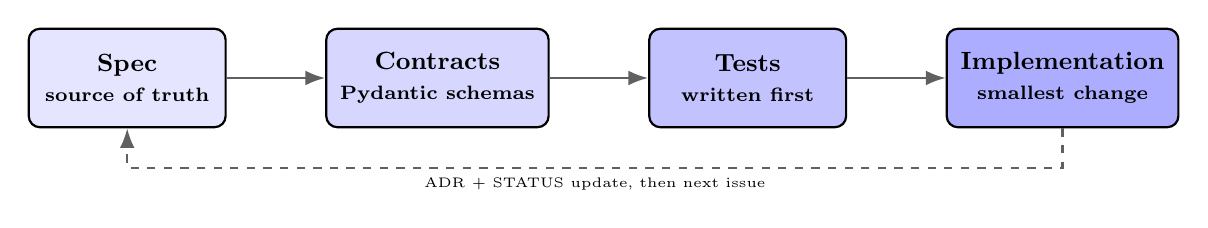
\begin{tikzpicture}[node distance=1.25cm]
    \node[stage,fill=blue!10] (p1) {Spec\\{\scriptsize source of truth}};
    \node[stage,fill=blue!16,right=of p1] (p2) {Contracts\\{\scriptsize Pydantic schemas}};
    \node[stage,fill=blue!24,right=of p2] (p3) {Tests\\{\scriptsize written first}};
    \node[stage,fill=blue!32,right=of p3] (p4) {Implementation\\{\scriptsize smallest change}};
    \draw[flow] (p1)--(p2);
    \draw[flow] (p2)--(p3);
    \draw[flow] (p3)--(p4);
    \draw[flow,dashed] (p4.south) -- ++(0,-0.5) -| (p1.south)
      node[pos=.25,below,font=\tiny]{ADR + STATUS update, then next issue};
  \end{tikzpicture}
  \vspace{0.3cm}
  \small
  Every decision that deviates from the specification is recorded in an Architecture
  Decision Record. The repository --- not a chat history --- is the memory between sessions.
\end{frame}

\begin{frame}{Project Management --- Task Table}
  \slidepurpose{Summarise work packages, duration and real progress}{Organisation / planning}
  \scriptsize
  \renewcommand{\arraystretch}{1.18}
  \begin{adjustbox}{max width=0.99\textwidth}
  \begin{tabular}{|c|p{5.9cm}|c|p{4.4cm}|}
    \hline
    \textbf{ID} & \textbf{Work package} & \textbf{Issues} & \textbf{State} \\ \hline
    \rowcolor{green!12} W1 & Framing, contracts, tooling, corpus & 8 & 5 closed \checkmark \\ \hline
    \rowcolor{green!12} W2 & Ingestion, embeddings, both indexes, access control & 7 & 4 closed \checkmark \\ \hline
    \rowcolor{green!8} W3 & VLM, citations, structured output, API/UI & 6 & 1 closed \\ \hline
    W4 & MCP server, workflow, budgets, approval, tickets & 5 & not started \\ \hline
    W5 & Reranker dataset, fine-tuning, evaluation, security suites & 6 & not started \\ \hline
    W6 & Benchmarks, Docker deployment, demo, deliverables & 5 & not started \\ \hline
    \hline
    \multicolumn{2}{|l|}{\textbf{Total backlog}} & \textbf{37} & \textbf{10 closed (27\,\%)} \\ \hline
  \end{tabular}
  \end{adjustbox}\par
  \vspace{0.2cm}
  \centering\tiny Work is tracked as GitHub Issues \#1--\#37 grouped into these six milestones.\par
\end{frame}

\begin{frame}{Project Management --- Gantt Chart}
  \slidepurpose{Project the validated tasks onto a readable timeline}{Organisation / planning}
  \centering
  \begin{adjustbox}{max width=0.98\textwidth,max totalheight=0.72\textheight}
  \begin{ganttchart}[
    hgrid,vgrid,x unit=.42cm,y unit chart=.62cm,y unit title=.5cm,
    title label font=\scriptsize\bfseries,bar label font=\scriptsize,
    bar/.append style={fill=blue!18,draw=blue!65!black},
    group/.append style={fill=black!10,draw=black!65},
    link/.style={-Latex,draw=black!60}]{1}{24}
    \gantttitle{Six-week plan}{24}\\
    \gantttitle{W1}{4}\gantttitle{W2}{4}\gantttitle{W3}{4}\gantttitle{W4}{4}\gantttitle{W5}{4}\gantttitle{W6}{4}\\
    \ganttgroup{Delivered}{1}{8}\\
    \ganttbar[name=w1,bar/.append style={fill=green!35,draw=green!55!black}]{$\checkmark$ W1 Framing \& contracts}{1}{4}\\
    \ganttbar[name=w2,bar/.append style={fill=green!35,draw=green!55!black}]{$\checkmark$ W2 Ingestion \& indexes}{5}{8}\\
    \ganttgroup{In progress}{9}{24}\\
    \ganttbar[name=w3,bar/.append style={fill=orange!35,draw=orange!65!black}]{W3 VLM \& citations}{9}{12}\\
    \ganttbar[name=w4]{W4 MCP \& workflow}{13}{16}\\
    \ganttbar[name=w5]{W5 Reranker \& evaluation}{17}{20}\\
    \ganttbar[name=w6]{W6 Deployment \& demo}{21}{24}\\
    \ganttlink{w1}{w2}\ganttlink{w2}{w3}\ganttlink{w3}{w4}\ganttlink{w4}{w5}\ganttlink{w5}{w6}
  \end{ganttchart}
  \end{adjustbox}
\end{frame}

\section{Design and Implementation}

\begin{frame}{Proposed Architecture}
  \slidepurpose{Show boundaries, components, data flow and responsibilities}{Design}
  \tikzsolutionfigure{
  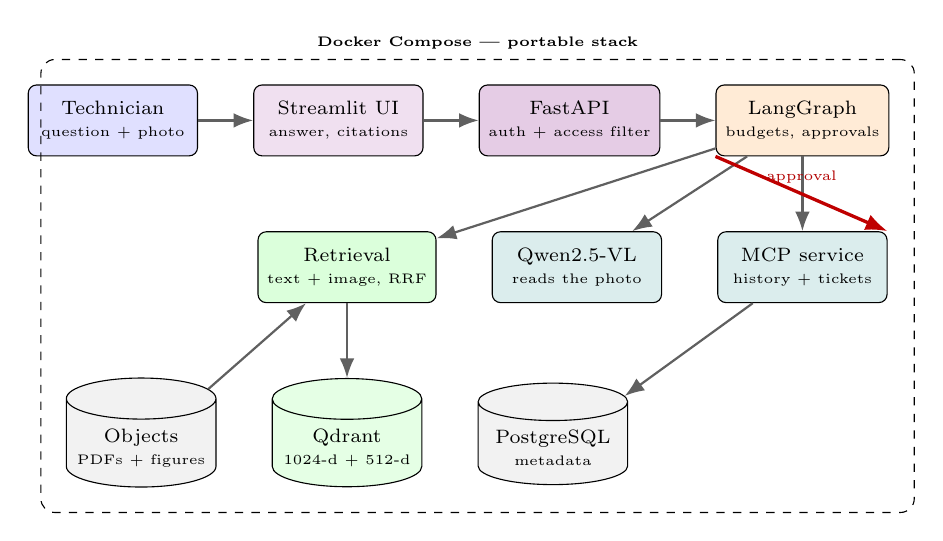
\begin{tikzpicture}[node distance=0.95cm and 0.7cm]
    \node[component,fill=blue!12] (user) {Technician\\\tiny question + photo};
    \node[component,fill=violet!12,right=of user] (ui) {Streamlit UI\\\tiny answer, citations};
    \node[component,fill=violet!20,right=of ui] (api) {FastAPI\\\tiny auth + access filter};
    \node[component,fill=orange!16,right=of api] (flow) {LangGraph\\\tiny budgets, approvals};
    \node[component,fill=teal!14,below=of flow] (mcp) {MCP service\\\tiny history + tickets};
    \node[component,fill=teal!14,left=of mcp] (vlm) {Qwen2.5-VL\\\tiny reads the photo};
    \node[component,fill=green!14,left=of vlm] (ret) {Retrieval\\\tiny text + image, RRF};
    \node[datastore,fill=green!10,below=of ret] (qd) {Qdrant\\\tiny 1024-d + 512-d};
    \node[datastore,fill=gray!10,left=of qd] (obj) {Objects\\\tiny PDFs + figures};
    \node[datastore,fill=gray!10,right=of qd] (pg) {PostgreSQL\\\tiny metadata};
    \draw[flow] (user)--(ui);
    \draw[flow] (ui)--(api);
    \draw[flow] (api)--(flow);
    \draw[flow] (flow)--(vlm);
    \draw[flow] (flow)--(mcp);
    \draw[flow] (flow)--(ret);
    \draw[flow] (ret)--(qd);
    \draw[flow] (obj)--(ret);
    \draw[flow] (mcp)--(pg);
    \draw[criticalflow] (flow.south west) -- node[above,font=\tiny,text=red!70!black]{approval} (mcp.north east);
    \node[boundary,fit=(api)(flow)(vlm)(mcp)(ret)(qd)(pg)(obj),label={[font=\tiny\bfseries]above:Docker Compose --- portable stack}] {};
  \end{tikzpicture}
  }{Component architecture. The access filter is applied inside the vector query, not after it.}
\end{frame}

\begin{frame}{Security Model --- Three Hard Boundaries}
  \slidepurpose{Explain the guarantees that are enforced by code, not by intent}{Design}
  \scriptsize
  \renewcommand{\arraystretch}{1.25}
  \begin{adjustbox}{max width=0.99\textwidth}
  \begin{tabular}{|p{4.0cm}|p{6.2cm}|p{3.0cm}|}
    \hline
    \textbf{Boundary} & \textbf{How it is enforced} & \textbf{Proven by} \\ \hline
    User/group $\rightarrow$ documents &
    Filter applied \emph{inside} the Qdrant query; deny by default, so an unlabelled
    document is visible to nobody &
    access-control tests \\ \hline
    Model $\rightarrow$ sensitive action &
    Approval token is a signed JWT bound to the user \emph{and} a SHA-256 of the exact
    content; single use, so a replay fails and any edit invalidates it &
    approval tests \\ \hline
    Document text $\rightarrow$ instructions &
    Retrieved text is delimited and declared untrusted; the prompt loader \emph{refuses
    to load} a prompt that does not delimit it &
    prompt-loader tests \\ \hline
  \end{tabular}
  \end{adjustbox}
  \vspace{0.15cm}
  \begin{alertblock}{Also enforced}
    \tiny A citation that was not actually retrieved, or that does not support its claim, cannot be produced: citations are built from the retrieved element itself. Opening a file checks permission \emph{before} reading a single byte, and an unknown document is denied rather than reported as missing --- otherwise it would be an enumeration oracle.
  \end{alertblock}
\end{frame}

\begin{frame}{Core Workflow}
  \slidepurpose{Explain the most important end-to-end interaction}{Implementation}
  \centering
  \begin{adjustbox}{max width=0.96\linewidth}
  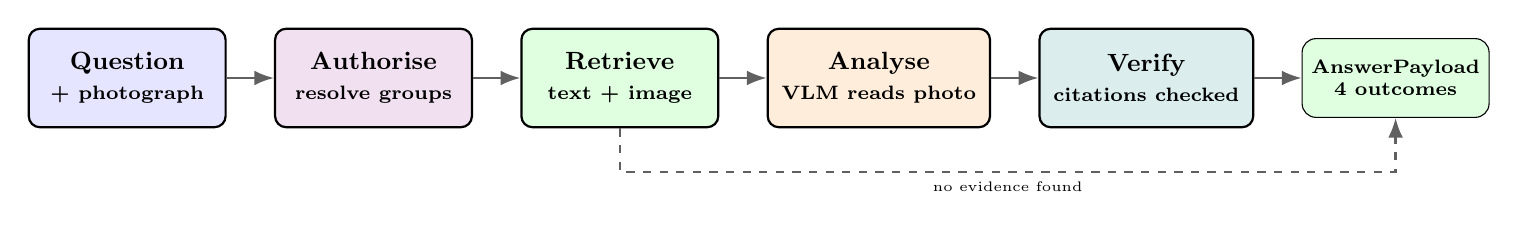
\begin{tikzpicture}[node distance=0.6cm]
    \node[stage,fill=blue!10] (s1) {Question\\{\scriptsize + photograph}};
    \node[stage,fill=violet!12,right=of s1] (s2) {Authorise\\{\scriptsize resolve groups}};
    \node[stage,fill=green!12,right=of s2] (s3) {Retrieve\\{\scriptsize text + image}};
    \node[stage,fill=orange!14,right=of s3] (s4) {Analyse\\{\scriptsize VLM reads photo}};
    \node[stage,fill=teal!14,right=of s4] (s5) {Verify\\{\scriptsize citations checked}};
    \node[result,right=of s5] (s6) {AnswerPayload\\{\scriptsize 4 outcomes}};
    \draw[flow] (s1)--(s2);
    \draw[flow] (s2)--(s3);
    \draw[flow] (s3)--(s4);
    \draw[flow] (s4)--(s5);
    \draw[flow] (s5)--(s6);
    \draw[flow,dashed] (s3.south) -- ++(0,-0.55) -| node[pos=.25,below,font=\tiny]{no evidence found}(s6.south);
  \end{tikzpicture}
  \end{adjustbox}
  \vspace{0.3cm}
  \small
  Budgets are enforced in code: at most 3 MCP calls, 6 model calls and 60 seconds per
  request. When the budget is exhausted the system abstains --- it does not improvise.
\end{frame}

\begin{frame}{Technology Choices}
  \slidepurpose{Connect each technology to a concrete responsibility}{Implementation}
  \centering
  \begin{adjustbox}{max width=0.98\linewidth}
  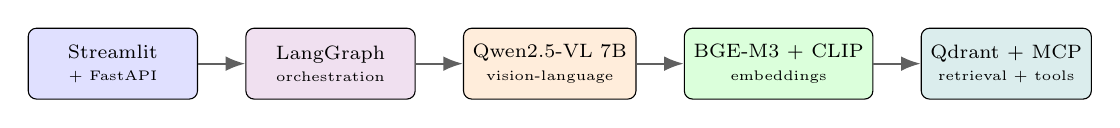
\begin{tikzpicture}[node distance=.6cm]
    \node[component,fill=blue!12] (t1) {Streamlit\\\tiny + FastAPI};
    \node[component,fill=violet!12,right=of t1] (t2) {LangGraph\\\tiny orchestration};
    \node[component,fill=orange!14,right=of t2] (t3) {Qwen2.5-VL 7B\\\tiny vision-language};
    \node[component,fill=green!14,right=of t3] (t4) {BGE-M3 + CLIP\\\tiny embeddings};
    \node[component,fill=teal!14,right=of t4] (t5) {Qdrant + MCP\\\tiny retrieval + tools};
    \draw[flow] (t1)--(t2);
    \draw[flow] (t2)--(t3);
    \draw[flow] (t3)--(t4);
    \draw[flow] (t4)--(t5);
  \end{tikzpicture}
  \end{adjustbox}
  \vspace{0.3cm}
  \small
  \begin{columns}[T]
    \begin{column}{0.48\textwidth}
      \begin{block}{\small Model choices}
        \tiny
        Qwen2.5-VL-7B-Instruct in 4-bit AWQ (fixed, never substituted) · BGE-M3, 1024-d
        multilingual text · CLIP ViT-B/32 image tower paired with a multilingual text
        tower, both licence-clean.
      \end{block}
    \end{column}
    \begin{column}{0.48\textwidth}
      \begin{block}{\small Infrastructure}
        \tiny
        Qdrant (vectors) · PostgreSQL (metadata) · object storage behind an interface ·
        MLflow (runs) · Docker Compose, so the stack runs on a machine with no GPU.
      \end{block}
    \end{column}
  \end{columns}
\end{frame}

\begin{frame}{What Was Actually Built}
  \slidepurpose{Map the implemented modules to their responsibility}{Implementation}
  \scriptsize
  \renewcommand{\arraystretch}{1.15}
  \begin{adjustbox}{max width=0.99\textwidth}
  \begin{tabular}{|p{4.1cm}|p{8.9cm}|}
    \hline
    \textbf{Module} & \textbf{Responsibility} \\ \hline
    \texttt{schemas} & Output contract: four statuses, citation model, status invariants, unknown fields rejected \\ \hline
    \texttt{security} & Deny-by-default identity, vector-query filter, content-bound approval tokens, replay protection \\ \hline
    \texttt{prompts} & Four versioned YAML prompts; loader rejects a prompt that does not delimit untrusted input \\ \hline
    \texttt{ingestion} & PDF $\rightarrow$ paragraphs, tables, figures and OCR text, each with full document metadata \\ \hline
    \texttt{retrieval} & BGE-M3 and CLIP embedders, two access-filtered indexes, RRF-ready rendering \\ \hline
    \texttt{vlm} & Provider protocol plus a deterministic, citation-safe stub (the real model is next) \\ \hline
    \texttt{runtime} & Device probe and a model ladder that explains every decision it makes \\ \hline
    \texttt{storage} & Object-store interface: filesystem today, S3-compatible next \\ \hline
    \texttt{corpus} & 34 synthetic manuals, 2 equipment families, reproducible byte for byte \\ \hline
  \end{tabular}
  \end{adjustbox}
\end{frame}

\section{Validation and Results}

\begin{frame}{Engineering Quality --- The Gate}
  \slidepurpose{Show the verification that every commit must pass}{Validation}
  \begin{columns}[T]
    \begin{column}{0.44\textwidth}
      \begin{block}{Automatic checks}
        \scriptsize
        \begin{itemize}
          \item \textbf{413 tests} pass, 41 of them against a live Qdrant container.
          \item \textbf{mypy --strict} clean on 32 modules.
          \item ruff lint and formatting clean.
          \item Secret scanning on every commit.
        \end{itemize}
      \end{block}
    \end{column}
    \begin{column}{0.52\textwidth}
      \begin{block}{Tests that defend the promises}
        \tiny
        \begin{itemize}
          \item An answer without a citation is rejected by the schema.
          \item A confidence field cannot exist: unknown fields are forbidden.
          \item A principal with no groups is \emph{refused}, not given an empty filter.
          \item A denied file open reads \textbf{zero bytes} --- asserted with a recording store.
          \item An approval token cannot be replayed, and editing the content invalidates it.
        \end{itemize}
      \end{block}
    \end{column}
  \end{columns}
  \vspace{0.2cm}
  \centering\scriptsize
  Documented divergences live in Architecture Decision Records: the task runner, the model ladder, the optional ML stack, the prompt format, object storage and the encoders.
\end{frame}

\begin{frame}{Measured Model Behaviour}
  \slidepurpose{Present verified measurements, including the uncomfortable one}{Validation}
  \scriptsize
  \renewcommand{\arraystretch}{1.2}
  \begin{adjustbox}{max width=0.98\textwidth}
  \begin{tabular}{|p{6.2cm}|c|c|}
    \hline
    \textbf{Check} & \textbf{Value} & \textbf{Verdict} \\ \hline
    BGE-M3 embedding width & 1024-d & as configured \\ \hline
    BGE-M3: related vs unrelated passage & 0.849 vs 0.459 & semantic \checkmark \\ \hline
    CLIP image width & 512-d & as configured \\ \hline
    CLIP: figure vs itself / vs another figure & 1.000 / 0.816 & image search sound \\ \hline
    \rowcolor{red!10} CLIP text$\rightarrow$image, \emph{correct} panel & 0.269 & --- \\ \hline
    \rowcolor{red!10} CLIP text$\rightarrow$image, \emph{wrong} panel & 0.299 & \textbf{wrong one wins} \\ \hline
  \end{tabular}
  \end{adjustbox}
  \vspace{0.2cm}
  \begin{alertblock}{Reported, not hidden}
    \tiny The last two rows are a real limitation: flat vector-drawn panels are far from the photographs CLIP was trained on, so cross-modal ranking does not hold on this corpus. Text$\rightarrow$image quality is therefore \emph{measured and reported separately} from image$\rightarrow$image, and the vision-language model reading the actual figure remains the primary path. A number that flatters the project is worth less than one that is true.
  \end{alertblock}
\end{frame}

\begin{frame}{Bugs Found by Executing, Not by Testing}
  \slidepurpose{Show that running the real stack found what doubles could not}{Validation}
  \scriptsize
  \renewcommand{\arraystretch}{1.2}
  \begin{adjustbox}{max width=0.99\textwidth}
  \begin{tabular}{|p{5.0cm}|p{4.0cm}|p{4.2cm}|}
    \hline
    \textbf{Symptom} & \textbf{Cause} & \textbf{Fix} \\ \hline
    Generated tables had no readable text at all & \texttt{insert\_textbox} writes \emph{nothing} when text overflows, returning a negative height & Measure and truncate, then draw with \texttt{insert\_text} \\ \hline
    Captions contained ``?'' instead of dashes & Built-in fonts cover Latin-1 only & Fail loudly on unrenderable characters \\ \hline
    \texttt{Torch not compiled with CUDA enabled} & A visible GPU plus a CPU-only torch build & Mark the device \emph{present but unusable}; never select it \\ \hline
    Embedding call crashed on a missing tensor & A major library version changed the return type & Read the pooled output explicitly; verify against real weights \\ \hline
  \end{tabular}
  \end{adjustbox}\par
  \vspace{0.15cm}
  \centering\tiny
  Each of these was invisible to unit tests written against stand-ins. They only surfaced when the real models and real PDFs ran --- which is precisely why they are now recorded in the handoff document.\par
\end{frame}

\begin{frame}{Project Progress}
  \slidepurpose{Give an honest completion figure per milestone}{Validation}
  \centering
  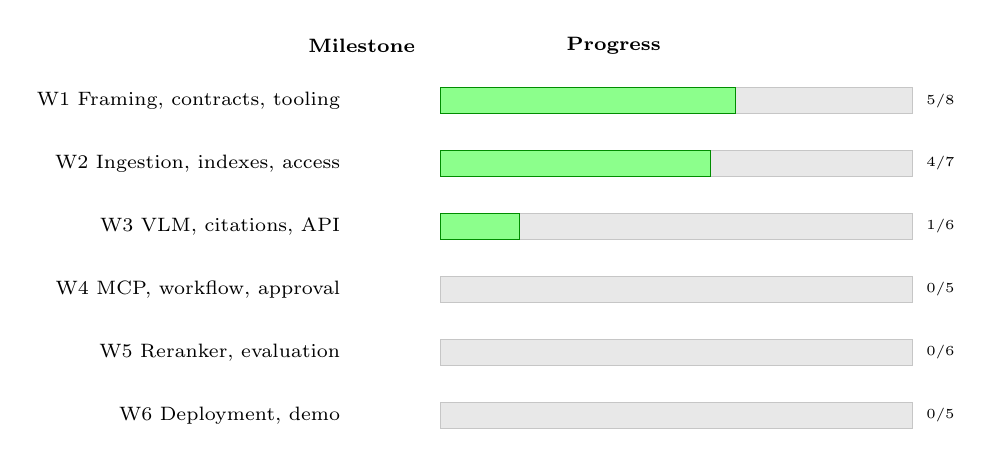
\begin{tikzpicture}[x=1cm,y=1cm]
    \node[font=\scriptsize\bfseries] at (-1.0,3.4) {Milestone};
    \node[font=\scriptsize\bfseries] at (2.2,3.4) {Progress};
    \foreach \y/\label/\done/\total in {%
      2.7/{W1 Framing, contracts, tooling}/{5}/{8},
      1.9/{W2 Ingestion, indexes, access}/{4}/{7},
      1.1/{W3 VLM, citations, API}/{1}/{6},
      0.3/{W4 MCP, workflow, approval}/{0}/{5},
      -0.5/{W5 Reranker, evaluation}/{0}/{6},
      -1.3/{W6 Deployment, demo}/{0}/{5}}{%
      \pgfmathsetmacro{\ylo}{\y-0.17}%
      \pgfmathsetmacro{\yhi}{\y+0.17}%
      \pgfmathsetmacro{\w}{\done*6.0/\total}%
      \node[anchor=east,font=\scriptsize] at (-1.15,\y) {\label};
      \fill[gray!18] (0,\ylo) rectangle (6.0,\yhi);
      \draw[gray!45] (0,\ylo) rectangle (6.0,\yhi);
      \ifdim\w pt>0.01pt
        \fill[green!45] (0,\ylo) rectangle (\w,\yhi);
        \draw[green!55!black] (0,\ylo) rectangle (\w,\yhi);
      \fi
      \node[font=\tiny] at (6.35,\y) {\done/\total};
    }
  \end{tikzpicture}
  \vspace{0.35cm}
  \begin{columns}[T]
    \begin{column}{0.32\textwidth}
      \centering\small\textbf{27\,\%}\\ \tiny of the backlog closed (10/37)
    \end{column}
    \begin{column}{0.32\textwidth}
      \centering\small\textbf{$\approx$30\,\%}\\ \tiny by estimated effort
    \end{column}
    \begin{column}{0.32\textwidth}
      \centering\small\textbf{0\,\%}\\ \tiny demoable end-to-end, for now
    \end{column}
  \end{columns}
\end{frame}

\section{Limits and Next Steps}

\begin{frame}{Known Limits --- Stated Plainly}
  \slidepurpose{Separate what works from what has never run}{Closure}
  \begin{columns}[T]
    \begin{column}{0.48\textwidth}
      \begin{block}{Works today}
        \scriptsize
        \begin{itemize}
          \item Corpus generation: 34 documents, reproducible.
          \item PDF ingestion with tables, figures and OCR hooks.
          \item Real embeddings loaded and measured.
          \item Access-filtered search, verified against live Qdrant.
          \item Approval tokens with replay protection.
        \end{itemize}
      \end{block}
    \end{column}
    \begin{column}{0.48\textwidth}
      \begin{alertblock}{Not yet true}
        \scriptsize
        \begin{itemize}
          \item \textbf{No question can be answered end to end yet.}
          \item The 7B vision-language model has never been loaded.
          \item OCR has never actually run (no Tesseract on the host).
          \item No Docker image or Compose file exists.
          \item No evaluation set, no fine-tuned reranker.
        \end{itemize}
      \end{alertblock}
    \end{column}
  \end{columns}
\end{frame}

\begin{frame}{Roadmap}
  \slidepurpose{Separate delivered scope from realistic future work}{Closure}
  \centering
  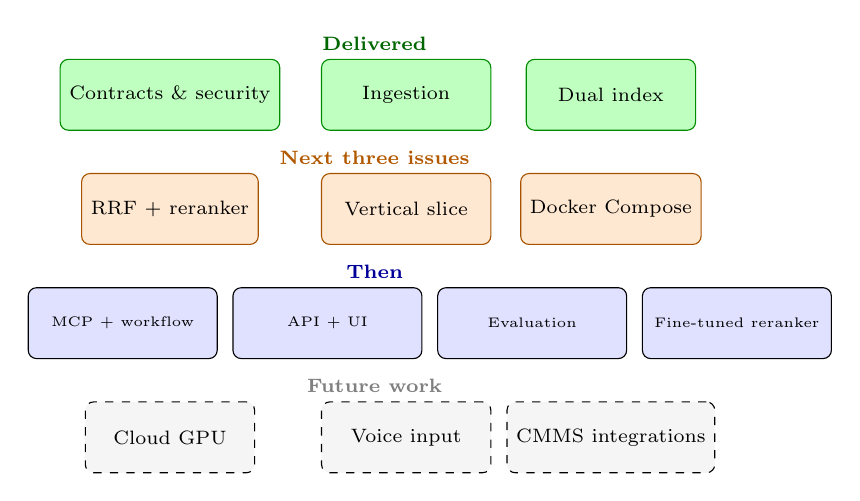
\begin{tikzpicture}[x=1cm,y=1cm]
    \node[font=\bfseries\scriptsize,green!40!black] at (4.0,2.5) {Delivered};
    \foreach \x/\label in {1.4/{Contracts \& security},4.4/{Ingestion},7.0/{Dual index}}
      \node[component,fill=green!25,draw=green!55!black] at (\x,1.85) {\label};
    \node[font=\bfseries\scriptsize,orange!70!black] at (4.0,1.05) {Next three issues};
    \foreach \x/\label in {1.4/{RRF + reranker},4.4/{Vertical slice},7.0/{Docker Compose}}
      \node[component,fill=orange!18,draw=orange!65!black] at (\x,0.4) {\label};
    \node[font=\bfseries\scriptsize,blue!60!black] at (4.0,-0.4) {Then};
    \foreach \x/\label in {0.8/{MCP + workflow},3.4/{API + UI},6.0/{Evaluation},8.6/{Fine-tuned reranker}}
      \node[component,font=\tiny,minimum width=2.4cm,fill=blue!12] at (\x,-1.05) {\label};
    \node[font=\bfseries\scriptsize,gray] at (4.0,-1.85) {Future work};
    \foreach \x/\label in {1.4/{Cloud GPU},4.4/{Voice input},7.0/{CMMS integrations}}
      \node[component,dashed,fill=gray!8] at (\x,-2.5) {\label};
  \end{tikzpicture}
\end{frame}

\begin{frame}{Conclusion}
  \slidepurpose{Close on the core value and the evidence}{Closure}
  \begin{alertblock}{Key Takeaway}
    MaintiDoc answers maintenance questions with evidence a technician can check --- and
    refuses to answer when it has none. Integrity was treated as an engineering
    requirement: the schema cannot carry a fabricated confidence score, a citation cannot
    point at an unretrieved page, and a file cannot be read before permission is checked.
  \end{alertblock}
  \vspace{0.25cm}
  \small
  \begin{itemize}
    \item \texttt{Contracts, security and retrieval core are built and verified: 413 tests.}
    \item \texttt{Real embeddings are loaded and measured, including a limitation that does not flatter the result.}
    \item \texttt{The remaining work is joined-up, not exploratory: workflow, tools, interfaces, deployment.}
  \end{itemize}
  \centering
  \vfill
  \Large Thank you --- Questions?
\end{frame}

\end{document}